\documentclass[10pt,a4paper]{report}
\usepackage{listings}
\usepackage{color}

\definecolor{dkgreen}{rgb}{0,0.6,0}
\definecolor{gray}{rgb}{0.5,0.5,0.5}
\definecolor{mauve}{rgb}{0.58,0,0.82}

\lstset{frame=tb,
  language=Java,
  aboveskip=3mm,
  belowskip=3mm,
  showstringspaces=false,
  columns=flexible,
  basicstyle={\small\ttfamily},
  numbers=none,
  numberstyle=\tiny\color{gray},
  keywordstyle=\color{blue},
  commentstyle=\color{dkgreen},
  stringstyle=\color{mauve},
  breaklines=true,
  breakatwhitespace=true,    
  tabsize=3
}
\usepackage[utf8]{inputenc}
\usepackage{float}
\usepackage{amsmath}
\usepackage{amsfonts}
\usepackage{amssymb}
\usepackage{graphicx}
\usepackage{lmodern}
\usepackage[left=2cm,right=2cm,top=2cm,bottom=2cm]{geometry}
\begin{document}
\author{Yapi Donatien Achou}
\title{MEK4430 Homework 2}
\maketitle

\section{Derivation of the holdup equation}
Consider the one-dimension two fluid mass momentum equation for the case of steady state, fully developed incompressible flow:

\begin{equation} \label{l}
A_{L}\frac{\partial P_{IL}}{\partial x}-\tau_{L}S_{L}+\tau_{I}S_{I}-\rho_{L}g\sin (\beta)  = 0
\end{equation}

\begin{equation} \label{g}
A_{G}\frac{\partial P_{IG}}{\partial x}-\tau_{G}S_{G}-\tau_{I}S_{I}-\rho_{G}g\sin (\beta)  = 0
\end{equation}
The interfacial shear is given by

\begin{equation}
\tau_{I} = \frac{1}{8}\rho_{G}f_{G}\bar{u}^{2}
\end{equation}
where the interfacial friction factor $f$ is given by
\begin{equation}
f_{I} = \theta f_{G}
\end{equation}
The interfacial boundary condition for pressure is given by
\begin{equation}\label{bc}
P_{LI} = P_{GI} = P_{I}
\end{equation}
 Inserting \ref{bc} in to \ref{l} and \ref{g} we get 
 
 \begin{equation} \label{l1}
A_{L}\frac{\partial P_{I}}{\partial x}-\tau_{L}S_{L}+\tau_{I}S_{I}-\rho_{L}g\sin (\beta)  = 0
\end{equation}

\begin{equation} \label{g1}
A_{G}\frac{\partial P_{I}}{\partial x}-\tau_{G}S_{G}-\tau_{I}S_{I}-\rho_{G}g\sin (\beta)  = 0
\end{equation}
Dividing \ref{l1} and \ref{g1} by $A_{L}$ and $A_{G}$ respectively we get

\begin{equation} \label{l2}
\frac{\partial P_{I}}{\partial x}-\frac{\tau_{L}S_{L}}{A_{L}}+\frac{\tau_{I}S_{I}}{A_{L}}-\frac{\rho_{L}g\sin (\beta)}{A_{L}}  = 0
\end{equation}

\begin{equation} \label{g2}
\frac{\partial P_{I}}{\partial x}-\frac{\tau_{G}S_{G}}{A_{G}}-\frac{\tau_{I}S_{I}}{A_{G}}-\frac{\rho_{G}g\sin (\beta)}{A_{G}}  = 0
\end{equation}
Multiplying equation \ref{g2} by -1 and adding \ref{l2} and \ref{g2} makes the interfacial pressure gradient fall out and we get the holdup equation:

\begin{equation}\label{he}
\left( \frac{\tau_{G}S_{G}}{A_{G}}-\frac{\tau_{L}S_{L}}{A_{L}}\right)+\tau_{I}S_{I}\left(   \frac{1}{A_{G}}+\frac{1}{A_{L}}   \right)+g\sin(\beta)\left( \frac{\rho_{G}}{A_{G}}-\frac{\rho_{L}}{A_{L}}       \right) = 0
\end{equation} 
Using the hydraulic approximation the liquid, gas and interfacial shear stress $\tau_{L}, \tau_{G}, \tau_{I}$ in equation \ref{he} are given by

\begin{equation}
\tau_{L} = \frac{1}{8}\rho_{L}f_{L}\bar{U_{L}}^{2} \nonumber
\end{equation}

\begin{equation}
\tau_{G} = \frac{1}{8}\rho_{G}f_{G}\bar{U_{G}}^{2} \nonumber
\end{equation}

\begin{equation}
\tau_{I} = \frac{1}{8}\rho_{G}\theta f_{G}(\bar{u_{G}}-\bar{u_{L}})^{2} \nonumber
\end{equation}

where the in-situ phase velocity are related to the superficial phase velocity as

\begin{equation}
\bar{U_{L}} = \frac{U_{SL}}{\alpha_{L}}
\end{equation}

\begin{equation}
\bar{U_{G}} = \frac{U_{SG}}{(1-\alpha_{L})}
\end{equation}

where $\alpha_{L}$ is the liquid holdup given by
\begin{equation}
\alpha_{L} = \frac{A_{L}}{A}
\end{equation}
\section{Computation of the liquid holdup}
\begin{figure}[H]
\centering
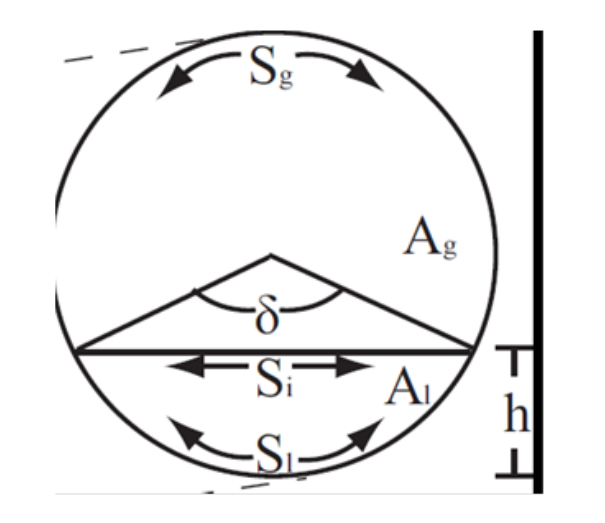
\includegraphics[scale=0.5]{h.png}
\caption{geometrycal variables}\label{visina8}
\end{figure}

Using $\theta = 1$ we derive the liquid holdup in this section. Given the following parameters:
\begin{equation}
\delta = 2\arccos\left(1-\frac{2h}{D} \right) \nonumber
\end{equation}

\begin{equation}
A = \frac{\pi D^{2}}{4}\nonumber
\end{equation}

\begin{equation}\label{al}
A_{L} = \frac{A}{2\pi}(\delta-\sin(\delta)) 
\end{equation}
\begin{equation}
A_{G} = A-A_{L} \nonumber
\end{equation}

\begin{equation}
S_{G} = D\left( \pi-\frac{\delta}{2}  \right) \nonumber
\end{equation}

\begin{equation}
S_{L} = \frac{D\delta}{2} \nonumber
\end{equation}

\begin{equation}
S_{I} = D\sin\left(\frac{\delta}{2}   \right) \nonumber
\end{equation}

\begin{equation}
D_{L} = \frac{4A_{L}}{S_{L}} \nonumber
\end{equation}

\begin{equation}
D_{L} = \frac{4A_{G}}{(S_{I}+S_{G})}\nonumber
\end{equation}

$\rho_{L} = 1000$ si, $\rho_{G} = 50$ si, $\mu_{L} = 0.001$ si, $\mu_{G} = 0.00001$ si are the physical properties of the phases.

The liquid holdup is by definition given by
\begin{equation}\label{holup}
\alpha_{L} = \frac{A_{L}}{A}
\end{equation}

and given the definition of $A_{L}$ from (\ref{al}) we get 
\begin{equation}\label{holdup2}
\alpha_{L} = \frac{\delta-\sin(\delta)}{2\pi}
\end{equation}
All the parameters in equation (\ref{he}) depend on $\delta$ so we can solve equation (\ref{he}) for $\delta$ and substitute it value in (\ref{holdup2}) to find the liquid holdup. To this end we implement a function in python called liquidHoldup() which solve equation (\ref{he}) for $\delta$ by using the bisection method for $0\leq \delta\leq \pi/2$. The liquid holdup is about
\begin{equation}
\alpha_{L} = 0.84 \nonumber
\end{equation}

the program out put:\\
parameters entered:\\
superficial liquid velocity $Usl =  0.3$\\
superficial gas velocity $Usg    =  3$\\
angle $\beta$                      =  0\\
$\theta$                           =  1\\
\\
computation results:\\
liquid holdup             = 0.837510724347\\
gas holdup                = 0.162489275653\\
\\
in-situ liquid velocity   = 0.358204368349 m/s\\
in-situ gas velocity      = 18.4627569293 m/s\\

\section{In-situ average phase velocities of gas and liquid  }
the in-situ average phase velocity are given by

\begin{equation}
\bar{U}_{L} = \frac{U_{sl}}{\alpha_{L}}
\end{equation}

\begin{equation}
\bar{U}_{G} = \frac{U_{sg}}{(1-\alpha_{L})}
\end{equation}
From the preview computation, $\alpha_{L} = 0.84$. with $U_{sl}=0.3$ $m/s$ and 
$U_{sg} = 3$ $m/s$. we get
\begin{equation}
U_{L} = 0.36\quad m/s \nonumber
\end{equation}

\begin{equation}
U_{G} = 18.5 \quad m/s \nonumber
\end{equation}

\section{Pressure gradient }
from equation (\ref{l2}) and (\ref{g2}) the pressure gradient is given by
\begin{equation}\label{ll}
\frac{\partial P_{I}}{\partial x}=\frac{\tau_{L}S_{L}}{A_{L}}-\frac{\tau_{I}S_{I}}{A_{L}}+\frac{\rho_{L}g\sin (\beta)}{A_{L}} 
\end{equation}

\begin{equation} \label{gg}
\frac{\partial P_{I}}{\partial x}=\frac{\tau_{G}S_{G}}{A_{G}}+\frac{\tau_{I}S_{I}}{A_{G}}+\frac{\rho_{G}g\sin (\beta)}{A_{G}}  
\end{equation} 

In both case the pressure gradient is about 

\begin{equation}
\frac{\partial P_{I}}{\partial x} = 173.2
\end{equation}

\section{Comparison of liquid hold up and in-situ velocities}

when $\theta$ is increased from 1 to 3 we have a very small change in liquid holdup and superficial velocities. This increase has little effect on the liquid holdup and the superficial velocities:\\
The out put of the program gives:
\\
\\
parameters entered:\\
superficial liquid velocity $Usl =  0.3$\\
superficial gas velocity $Usg    =  3$\\
angle $\beta$                      =  0\\
$\theta$                           =  1\\
\\
computation results:\\
liquid holdup             = 0.837510724346\\
gas holdup                = 0.162489275654\\
\\
in-situ liquid velocity   = 0.358204368349 m/s\\
in-situ gas velocity      = 18.4627569292 m/s\\




\clearpage
parameters entered:\\
superficial liquid velocity $Usl =  0.3$\\
superficial gas velocity $Usg    =  3$  \\
angle $\beta$                    =  0  \\
$\theta$                         =  3\\
\\
computation results:\\
liquid holdup             = 0.837105384959\\
gas holdup                = 0.162894615041\\
\\
in-situ liquid velocity   = 0.35837781645 m/s\\
in-situ gas velocity      = 18.4168150632 m/s\\
\\
The liquid hold up decrease by about $4*10^{-4}$ while the in-situ phase velocity of liquid increase by about $2*10^{-4}$ and the in-situ phase velocity of gas decrease by about $4.5*10^{-2}$. We can say that there is a very small change in the liquid holdup and the in-situ phase velocity when $\theta$ changes from 1 to 3

\section{Increasing the gas superficial phase velocity}
By doubling the gas superficial velocity we observe a decrease in the liquid holdup. Since the gas is moving faster in the pipe, to maintain the mass flow rate constant, the liquid level must decrease. \\
\\
program output:\\
parameters entered:\\
superficial liquid velocity $Usl =  0.3$\\
superficial gas velocity $Usg    =  6$\\
angle $\beta$                      =  0\\
$\theta$                           =  1\\

computation results:\\
liquid holdup             = 0.696680891221\\
gas holdup                = 0.303319108779\\
\\
in-situ liquid velocity   = 0.4306132173 m/s\\
in-situ gas velocity      = 19.7811474 m/s\\

the liquid holdup decrease by 0.14

\section{Change in liquid holdup by increasing the angle}
for $\theta = 10$ the liquid holdup is very small : 0.004. The gas occupied all the pipe according to the simulation result. This correspond to annular flow regime where the gas occupied most of the pipe. Bellow is the computation result:\\
\\
parameters entered:\\
superficial liquid velocity $Usl =  0.3$\\
superficial gas velocity $Usg    =  3$\\
angle $\beta$                      =  10\\
$\theta$                           =  1\\
\\
computation results:\\
liquid holdup             = 0.00371854672427\\
gas holdup                = 0.996281453276\\
\\
in-situ liquid velocity   = 80.6766788869 m/s\\
in-situ gas velocity      = 3.01119727777 m/s\\
\\
The gas superficial velocity is equal to the gas in-situ velocity. This is because the gas occupied all the pipe. Furthermore according $\alpha_{G} \approx 1$ 
\begin{equation}
U_{G} = \frac{U_{sg}}{\alpha_{G}}=U_{sg} \nonumber
\end{equation}
The liquid in-situ velocity is higher than it superficial velocity. Recall that the in-situ velocity of liquid is
\begin{equation}
U_{L} = \frac{Q_{L}}{A_{L}} = \frac{U_{sl}}{\alpha_{L}}\nonumber
\end{equation}
Since the liquid holdup decrease, the cross sectional areal of liquid decrease as well. To maintain a constant mass flow $Q_{L}$, the in-situ velocity must increase. Similarly since the holdup decrease, to maintain a constant superficial velocity $U_{sl}$, the in-situ velocity $U_{L}$ must increase





\section{python program}

In the program, the python function bisect() is used for root finding:
\begin{lstlisting}
"""
solve the holdup equation for sigma

"""
import numpy as np
import pylab as pl
from math import pi, sin, cos
from scipy.optimize import fsolve, bisect

def liquidHoldup(theta,Usg,Usl,beta,string=None):
    """
    this function takes as input the parameters theta 
    the superficial velocity of liquid and gas: Usl, Usg 
    and the string "print".
    
    usage: 
    to print results, enter the string "print":
    
    thata = 1; Usg = 3; Usl = 0.3; beta = 0
    liquidHoldup(thata,Usg,Usl,beta,"print")
    
    output:
    ################################################
    parameters entered:
    superficial liquid velocity Usl =  0.3
    superficial gas velocity Usg    =  3
    angle beta                      =  0
    #################################################
    computation results:
    liquid holdup             = 0.837510724346
    gas holdup                = 0.162489275654
    
    in-situ liquid velocity   = 0.358204368349 m/s
    in-situ gas velocity      = 18.4627569292 m/s
    ################################################
    
    to return the value of sigma to be used later in a computation:
    do not specify the string print:
    
    usage:
    sigma = liquidHoldup(thata,Usg,Usl,beta)

    """
    
    def holdupEquation(sigma):
        """
        This function return the holdup equation as a function of
        sigma. The holdup equation is used as an input
        by the fsolve() python function to return sigma.
        the python function fsolve() solves nonlinear equation.
        """
        #physical parameter values
        rhoL, rhoG = 1000, 50       # density

        D          = 0.1              # pipe diameter
        muL, muG   = 0.001, 0.00001 # dynamic viscosity
    
        # in-situ velocity
        alphaL = (sigma-sin(sigma))/(2*pi)
        UL = Usl/(alphaL)
        UG = Usg/(1-alphaL)
        
        # physical boundary of the pipe
        A  = (pi*D**2)/4                    # cross sectional area of pip
        AL = (A/2*pi)*(sigma-sin(sigma))    # cross sectional area of liquid
        AG = A-AL                           # cross sectional area of gas
        
        SL = (D*sigma)/2  
        SG = D*(pi-0.5*sigma)
        SI = D*sin(0.5*sigma)
        
        DL = (4*AL)/SL
        DG = (4*AG)/(SI+SG)               
        
        #shear stress
        ReG = (rhoG*UG*DG)/muG # gas Reynold number
        ReL = (rhoL*UL*DL)/muL # liquid Reynold number
    
        #blasius friction factor
        fG = 0.316/(ReG**0.25)            # gas friction factor
        fL = 0.316/(ReL**0.25)            # liquid friction factor
    
        #shear stress
        tauG = (1./8)*rhoG*fG*UG**2         # gas shear sress
        tauL = (1./8)*rhoL*fL*UL**2         # liquid shear stress
        tauI = (1./8)*rhoG*theta*fG*(UL-UG)**2    # interfacial shear stress
        g = 9.81 # gavitational constant
        
        #holdup equation as a function of sigma
        equation = ( ((tauG*SG)/AG)-((tauL*SL)/AL)   ) + tauI*SI*((1./AG)+(1./AL) )+g*sin(beta)*((rhoG/AG)-(rhoL/AL) )
        return equation
    

    sig = bisect(holdupEquation,0.1,pi/2.)
    #sig = fsolve(holdupEquation,0.8)
     
    #compute liquid holdup
    alphaL = (sig-sin(sig))/2.*pi
     
    #compute in-situ velocities
    UL = Usl/alphaL
    UG = Usg/(1-alphaL)
     
    #print result if string print is an iput to function liquidHolup()
    if string !=None:
        print"################################################"
        print"parameters entered:"
        print"superficial liquid velocity Usl = ", Usl
        print"superficial gas velocity Usg    = ", Usg
        print"angle beta                      = ", beta
        print"theta                           = ", theta
        print"#################################################"
        print"computation results:"
        print"liquid holdup             =", alphaL
        print"gas holdup                =", 1-alphaL
        print""
        print"in-situ liquid velocity   =",UL, "m/s"
        print"in-situ gas velocity      =",UG, "m/s"
        print"################################################"
        print"h", (0.1/2)*(1-cos(sig/2))
         
         
    
    return sig
    

def pressureGradient():
    """
    given the sigma compute the pressure gradient
    """
    theta, Usg, Usl, beta = 1,3,0.3,0
    sigma = liquidHoldup(theta,Usg,Usl,beta)
    rhoL, rhoG = 1000, 50       # density

    D          = 0.1              # pipe diameter
    muL, muG   = 0.001, 0.00001 # dynamic viscosity
    
    # in-situ velocity
    alphaL = (sigma-sin(sigma))/(2*pi)
    UL = Usl/(alphaL)
    UG = Usg/(1-alphaL)
        
    # physical boundary of the pipe
    A  = (pi*D**2)/4                    # cross sectional area of pip
    AL = (A/2*pi)*(sigma-sin(sigma))    # cross sectional area of liquid
    AG = A-AL                           # cross sectional area of gas
        
    SL = (D*sigma)/2  
    SG = D*(pi-0.5*sigma)
    SI = D*sin(0.5*sigma)
        
    DL = (4*AL)/SL
    DG = (4*AG)/(SI+SG)               
        
    #shear stress
    ReG = rhoG*UG*DG/muG # gas Reynold number
    ReL = rhoL*UL*DL/muL # liquid Reynold number
    print ReG,ReL
    
    fG = 0.316/(ReG**0.25)            # gas friction factor
    fL = 0.316/(ReL**0.25)            # liquid friction factor
    
    tauG = (1./8)*rhoG*fG*UG**2         # gas shear sress
    tauL = (1./8)*rhoL*fL*UL**2         # liquid shear stress
    tauI = (1./8)*rhoG*theta*fG*(UL-UG)**2    # interfacial shear stress
    g = 9.81 # gavitational constant
    
    PLI = (1./AL)*(tauL*SL-tauI*SI) +(rhoL*g*sin(beta))/(AL)
        
    PGI = (1./AG)*(tauG*SG+tauI*SI) +(rhoG*g*sin(beta))/(AG)
    
    print"parameters used for computation:"
    print"theta = ", theta
    print"Usl   = ", Usl
    print"Usg   = ", Usg
    print"beta  = ", beta
    print"##################################################"
    print"pressure gradient for liquid dPLi/dx", PLI
    print"pressure gradient for Gas dPGi/dx   ", PGI
    print"###################################################"
    print"DL",DL
    print"DG", DG

        
        
    
#pressureGradient()
theta, Usg,Usl,beta = 1,3,0.3,10
liquidHoldup(theta,Usg,Usl,beta,"print")




    
    
    
    


\end{lstlisting}

\end{document}